% Cover
\imprimircapa

% False cover sheet
%\imprimirfalsafolhaderosto

% Cover sheet
\imprimirfolhaderosto

% Card Catalog
\begin{fichacatalografica}
	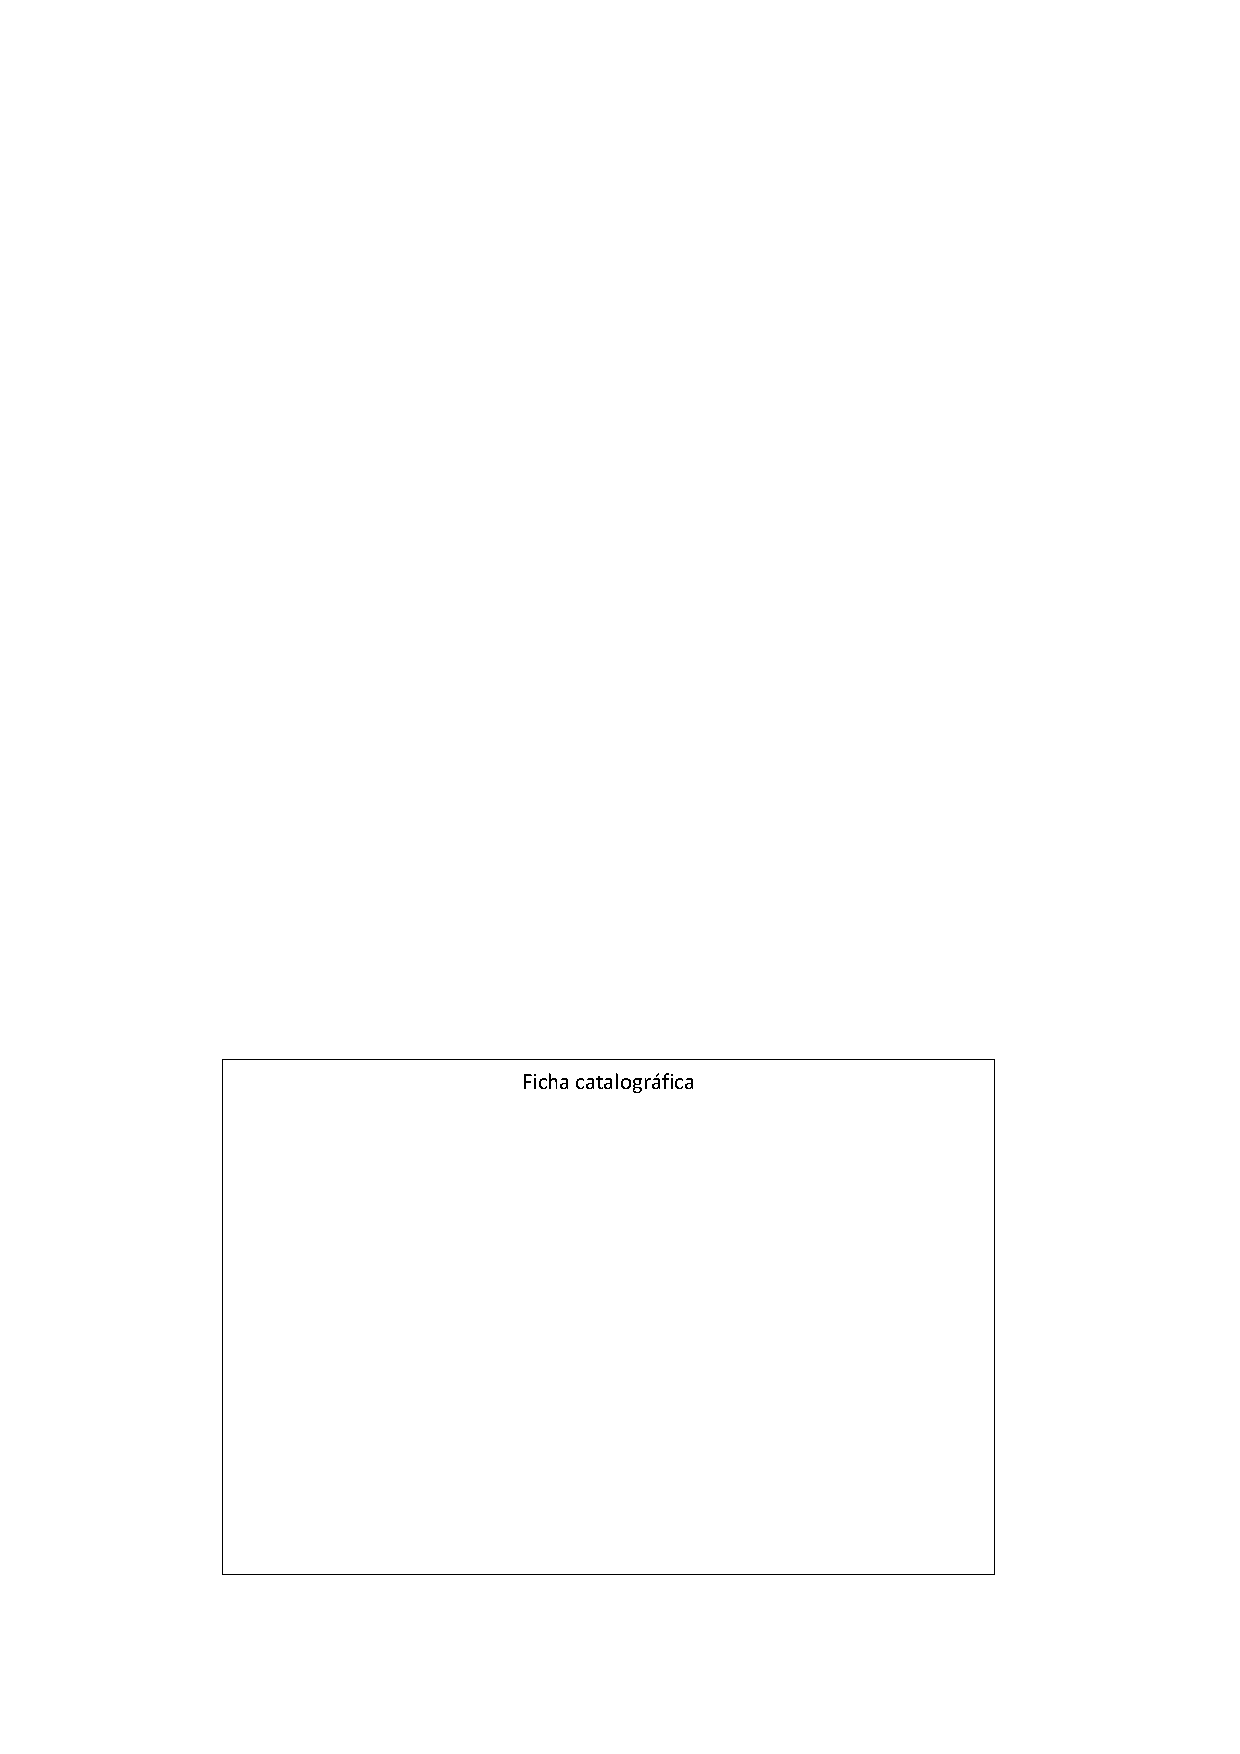
\includepdf{card-catalog.pdf}
\end{fichacatalografica}

% Approval sheet
%\begin{folhadeaprovacao}
%	
%	\begin{center}
%		{\ABNTEXchapterfont\large\imprimirautor}
%		
%		\vspace*{\fill}\vspace*{\fill}
%		\begin{center}
%			\ABNTEXchapterfont\bfseries\Large\imprimirtitulo
%		\end{center}
%		\vspace*{\fill}
%		
%		\hspace{.45\textwidth}
%		\begin{minipage}{.5\textwidth}
%			\imprimirpreambulo
%		\end{minipage}%
%		\vspace*{\fill}
%	\end{center}
%	
%	%Trabalho aprovado. \imprimirlocal, 31 de dezembro de 2020:
%	
%	\assinatura{\textbf{\imprimirorientador} \\ Orientador} 
%	\assinatura{\textbf{\imprimircoorientador} \\ Coorientador} 
%	\assinatura{\textbf{A} \\ Convidado 1}
%	\assinatura{\textbf{B} \\ Convidado 2}
%	
%	\begin{center}
%		\vspace*{0.5cm}
%		{\large\imprimirlocal}
%		\par
%		{\large\imprimirdata}
%		\vspace*{1cm}
%	\end{center}
%	
%\end{folhadeaprovacao}

% Abstract - Portuguese
\setlength{\absparsep}{18pt} % Spacing
\begin{resumo}
	Resumo do trabalho
	
	\vspace{\onelineskip}
	
	\noindent
	\textbf{Palavras-chave}: Indústria 4.0. RAMI4.0. Memória digital do produto. Arquitetura orientada a serviços (SOA). Cadeia de suprimentos.
\end{resumo}

% Abstract - English
\begin{resumo}[Abstract]
	\begin{otherlanguage*}{english}
		Abstract.
		
		\vspace{\onelineskip}

		\noindent 
		\textbf{Keywords}: Industry 4.0. RAMI4.0. Digital product memory. Service-oriented architecture (SOA). Supply chain. 
	\end{otherlanguage*}
\end{resumo}

% List of illustrations
\pdfbookmark[0]{\listfigurename}{lof}
\listoffigures*
\cleardoublepage

% List of tables
\pdfbookmark[0]{\listtablename}{lot}
\listoftables*
\cleardoublepage

% List of abbreviations and acronyms
\begin{siglas}
	\item[AAS] \textit{Asset Administration Shell} (Casca Administrativa do Ativo)
	\item[API] \textit{Application Programming Interface} (Interface de Programação de Aplicação)
	\item[BD] Banco de Dados
	\item[BI] \textit{Business Intelligence} (Inteligência Empresarial)

\end{siglas}

% Summary
\pdfbookmark[0]{\contentsname}{toc}
\tableofcontents*
\cleardoublepage
